% \documentclass{standalone}
%  \input{../tikz_header.tex}
 
%  \begin{document}
 

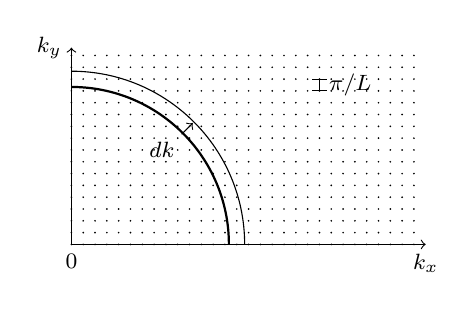
\begin{tikzpicture}[font=\footnotesize]

%\useasboundingbox (-1.3,-1.2) rectangle (11.2,4.7); 
%	\draw (0,0) rectangle (5,3);

  
%\clip (-26mm,-16mm) rectangle  (26mm, 16mm);  
   
 \foreach \u in {0,1,...,29}{%  
     \foreach \v in {0,1,...,16}{%  
          \draw[fill=gray]  (\u * 1.5mm,\v * 1.5mm)  circle (0.02mm) ;  
     }
  }
  
   \draw [ |-| ] ( 21 * 1.5mm, 13 * 1.5mm) -- node[right] { $\pi / L$} ++ (0, 1.5mm);
  
  
\draw[->] (0,0) -- (4.5,0) node [below] {$k_x$};  
  \draw[->] (0,0) -- (0,2.5) node [left] {$k_y$};  

  \draw[thick] (2,0) arc (0:90:2);
  \draw (2.2,0) arc (0:90:2.2);


%\draw[thick] (0,0) circle (1.9cm and 0.9cm);
%\draw[] (0,0) circle (2.1cm and 1.2cm);

%\node at (-10mm, 5mm) {$S(\omega)$};
%\node at (-15mm, 12.5mm) {$S(\omega + d\omega)$};
\node[below] at (0,0) {$0$};


\draw[->] (14mm,14mm) -- node (a) {} ++ (45:2mm);
%\draw[->] (10mm,8mm) -- ++ (-17:2mm);

\node at (11.5mm, 12mm) {$dk$};
%\node at (10mm, 5.5mm) {$dS_\omega$};



  
  \end{tikzpicture}



  %\end{document}
